\documentclass[letterpaper, 11pt]{extarticle}
% \usepackage{fontspec}

% ==================================================

% document parameters
% \usepackage[spanish, mexico, es-lcroman]{babel}
\usepackage[english]{babel}
\usepackage[margin = 1in]{geometry}

% ==================================================

% Packages for math
\usepackage{mathrsfs}
\usepackage{amsfonts}
\usepackage{amsmath}
\usepackage{amsthm}
\usepackage{amssymb}
\usepackage{physics}
\usepackage{dsfont}
\usepackage{esint}

% ==================================================

% Packages for writing
\usepackage{enumerate}
\usepackage[shortlabels]{enumitem}
\usepackage{framed}
\usepackage{csquotes}

% ==================================================

% Miscellaneous packages
\usepackage{float}
\usepackage{tabularx}
\usepackage{xcolor}
\usepackage{multicol}
\usepackage{subcaption}
\usepackage{caption}
\captionsetup{format = hang, margin = 10pt, font = small, labelfont = bf}

% Citation
\usepackage[round, authoryear]{natbib}

% Hyperlinks setup
\usepackage{hyperref}
\definecolor{links}{rgb}{0.36,0.54,0.66}
\hypersetup{
   colorlinks = true,
    linkcolor = black,
     urlcolor = blue,
    citecolor = blue,
    filecolor = blue,
    pdfauthor = {Author},
     pdftitle = {Title},
   pdfsubject = {subject},
  pdfkeywords = {one, two},
  pdfproducer = {LaTeX},
   pdfcreator = {pdfLaTeX},
   }
\usepackage{titlesec}
\usepackage[many]{tcolorbox}
\usepackage{chngcntr}

% Adjust spacing after the chapter title
\titlespacing*{\chapter}{0cm}{-2.0cm}{0.50cm}
\titlespacing*{\section}{0cm}{0.50cm}{0.25cm}

% Indent 
\setlength{\parindent}{0pt}
\setlength{\parskip}{1ex}

% Reset problem numbering per chapter
\newcounter{problem}[section]
\renewcommand{\theproblem}{\arabic{problem}}  % Flat numbering: 1, 2, 3...

\newtcbtheorem[use counter=problem]{problem}{Problem}%
    {enhanced,
    colback = black!5,
    colbacktitle = black!5,
    coltitle = black,
    boxrule = 0pt,
    frame hidden,
    borderline west = {0.5mm}{0.0mm}{black},
    fonttitle = \bfseries\sffamily,
    breakable,
    before skip = 5ex,
    after skip = 3ex,
    width = \linewidth,
}{problem}

\tcbuselibrary{skins, breakable}

% --- Basic commands ---
%   Euler's constant
\newcommand{\eu}{\mathrm{e}}

%   Imaginary unit
\newcommand{\im}{\mathrm{i}}

%   Sexagesimal degree symbol
\newcommand{\grado}{\,^{\circ}}

% --- Comandos para álgebra lineal ---
% Matrix transpose
\newcommand{\transpose}[1]{{#1}^{\mathsf{T}}}

%%% Comandos para cálculo
%   Definite integral from -\infty to +\infty
\newcommand{\Int}{\int\limits_{-\infty}^{\infty}}

%   Indefinite integral
\newcommand{\rint}[2]{\int{#1}\dd{#2}}

%  Definite integral
\newcommand{\Rint}[4]{\int\limits_{#1}^{#2}{#3}\dd{#4}}

%   Dot product symbol (use the command \bigcdot)
\makeatletter
\newcommand*\bigcdot{\mathpalette\bigcdot@{.5}}
\newcommand*\bigcdot@[2]{\mathbin{\vcenter{\hbox{\scalebox{#2}{$\m@th#1\bullet$}}}}}
\makeatother

%   Hamiltonian
\newcommand{\Ham}{\hat{\mathcal{H}}}

%   Trace
\renewcommand{\Tr}{\mathrm{Tr}}

% Christoffel symbol of the second kind
\newcommand{\christoffelsecond}[4]{\dfrac{1}{2}g^{#3 #4}(\partial_{#1} g_{#2 #4} + \partial_{#2} g_{#1 #4} - \partial_{#4} g_{#1 #2})}

% Riemann curvature tensor
\newcommand{\riemanncurvature}[5]{\partial_{#3} \Gamma_{#4 #2}^{#1} - \partial_{#4} \Gamma_{#3 #2}^{#1} + \Gamma_{#3 #5}^{#1} \Gamma_{#4 #2}^{#5} - \Gamma_{#4 #5}^{#1} \Gamma_{#3 #2}^{#5}}

% Covariant Riemann curvature tensor
\newcommand{\covariantriemanncurvature}[5]{g_{#1 #5} R^{#5}{}_{#2 #3 #4}}

% Ricci tensor
\newcommand{\riccitensor}[5]{g_{#1 #5} R^{#5}{}_{#2 #3 #4}}
\usepackage{svg} 
\usepackage{graphicx}
\graphicspath{{./images/}}

\usepackage{makeidx}
\usepackage{listings}
\usepackage{courier} 
\lstset{
  basicstyle=\ttfamily\small,
  columns=fullflexible,
  frame=single,
  breaklines=true,
  showstringspaces=false,
  tabsize=2,
  xleftmargin=2em
}

\makeindex

\begin{document}

% -------------------------------------- FRONT PAGE ------------------------------------------------
\begin{center}
  \includesvg[scale=0.5]{logo} 
\end{center}


\begin{center}
  \Huge{{\textbf{DEPARTMENT OF
  COMPUTER SCIENCE}}}
\end{center}


\begin{center}
  \large\textbf{The University of Chittagong}
\end{center}

{\vspace{1em}}

\begin{center}
  \begin{tabular}{|lp{10.0cm}lll|}
    \hline

    &  &  &  & \\
    &  &  &  & \\
    \textbf{Student Name:} & Sumaiya Tabassum
    
    \  &  &  &  \\
    \textbf{Student ID:} & 23701025

    \  &  &  & \\
    \textbf{Session:} & 2022-2023
    
    \  &  &  & \\
    \textbf{Course Title:} & Database Systems
    
    \  &  &  & \\
    \textbf{Course Code:} & CSE 413

    \  &  &  & \\
    \textbf{Task:} & Assignment 01 - Oracle Database 11g: SQL
Fundamentals I 

Chap 01 - 04 Exercise
    
    \  &  &  & \\
    \textbf{Submitted to:} & Rudra Pratap Deb Nath,
    
    Associate Professor,
    
    Department of Computer Science and Engineering
    
    \  &  &  & \\
    \textbf{Submitted Date:} & \today
    \
    
    \  &  &  & \\
    \hline
  \end{tabular}
\end{center}

\


% ----------------------------------------- INDEX PAGE ----------------------------------------------
\newpage
\tableofcontents
\newpage

% ---------------------------------------- MAIN CONTENT ---------------------------------------------

% ----------------------- Chapter 01 --------------------
\section*{Chapter 01}
\phantomsection
\addcontentsline{toc}{section}{Chapter 01: Retrieving Data Using the SQL \texttt{SELECT} Statement}

% ------ 1 -----------
\begin{problem}{}{problem-label}
    \textbf{Q:} \text{The following SELECT statement executes successfully:}
\begin{lstlisting}[language=SQL]
SELECT last_name, job_id, salary AS Sal
FROM employees;
\end{lstlisting}
    \vspace{1em}
    \textbf{A:} \text{True.}
    
\end{problem}

% ------ 2 -----------
\begin{problem}{}{problem-label}
    \textbf{Q:} \text{The following SELECT statement executes successfully:}
\begin{lstlisting}[language=SQL]
SELECT *
FROM job_grades;
\end{lstlisting}
    \vspace{1em}
    \textbf{A:} \text{False.}
    
\end{problem}

% ------ 3 -----------
\begin{problem}{}{problem-label}
    \textbf{Q:} \text{There are four coding errors in this statement. Can you identify them?}

    \begin{lstlisting}[language=SQL]
SELECT employee_id, last_name
sal x 12 ANNUAL SALARY
FROM employees;
    \end{lstlisting}
    \vspace{1em}
    \textbf{A:} 
    \begin{lstlisting}[language=SQL]
SELECT employee_id, last_name,
salary*12 "ANNUAL SALARY"
FROM hr.employees;
\end{lstlisting}
    
\end{problem}

% ------ 4 -----------
\newpage
\begin{problem}{}{problem-label}
    \textbf{Q:} \text{Your first task is to determine the structure of the \texttt{DEPARTMENTS} table and its contents.}
    
\begin{center}
  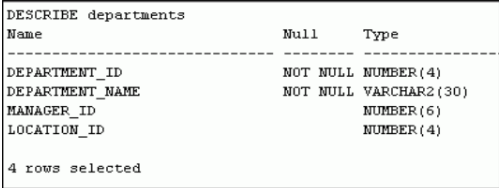
\includegraphics[scale=0.6]{images/c1q4.png}
\end{center}
\begin{center}
  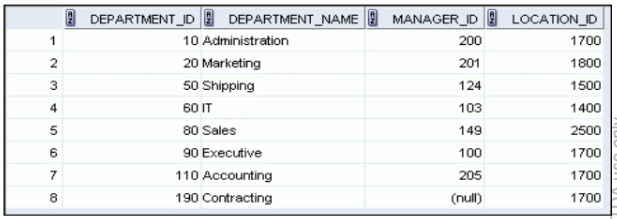
\includegraphics[scale=0.5]{images/c1q4-2.png}
\end{center}

    \vspace{1em}
    \textbf{A:} 
    \begin{lstlisting}[language=SQL]
DESCRIBE DEPARTMENTS
SELECT *
FROM hr.EMPLOYEES;
\end{lstlisting}

\vspace{1em}
\begin{center}
  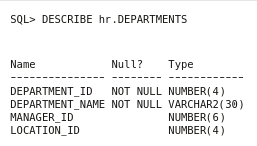
\includegraphics[scale=0.7]{images/c1a6-1.png}
\end{center}

\begin{center}
  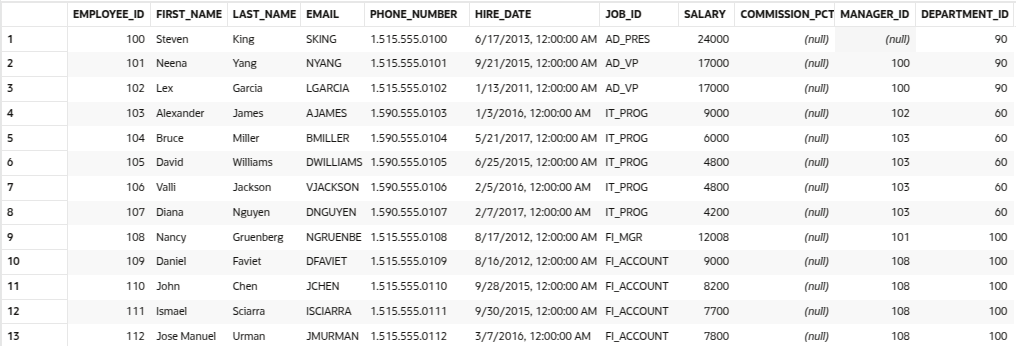
\includegraphics[scale=0.4]{images/c1a6-2.png}
\end{center}

    
\end{problem}


% ------ 5 -----------
\begin{problem}{}{problem-label}
    \textbf{Q:} \text{Your task is to determine the structure of the \texttt{EMPLOYEES} table}

\begin{center}
  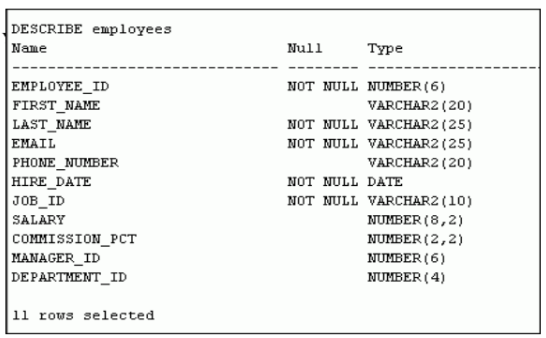
\includegraphics[scale=0.7]{images/c1q05.png}
\end{center}

    \vspace{1em}
    \textbf{A:}

    \vspace{1em}
    \begin{lstlisting}[language=SQL]
DESCRIBE hr.employees;
\end{lstlisting}
\begin{center}
  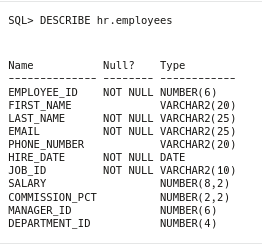
\includegraphics[scale=0.75]{images/c1a5.png}
\end{center}
    
\end{problem}

% ------ 6 -----------
\begin{problem}{}{problem-label}
\begin{tabular}{@{}l p{0.9\linewidth}@{}}
    \textbf{Q:} & The HR department wants a query to display the last name, job ID, hire date, and employee ID for each employee, with the employee ID appearing first. Provide an alias \texttt{STARTDATE} for the \texttt{HIRE\_DATE} column. Save your SQL statement to a file named \texttt{lab\_01\_05.sql} so that you can dispatch this file to the HR department.
    Test your query in the \texttt{lab\_01\_05.sql} file to ensure that it runs correctly.
\end{tabular}

\begin{center}
  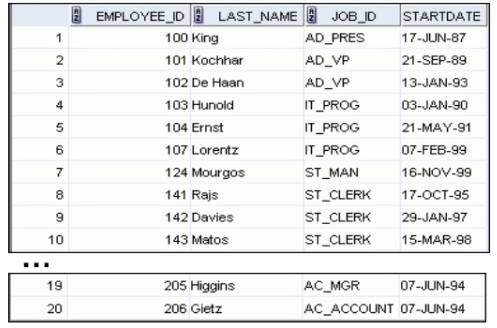
\includegraphics[scale=0.7]{images/c1q06.png}
\end{center}

    \vspace{1em}
    \begin{tabular}{@{}l p{0.9\linewidth}@{}}
  \textbf{A:} &
\end{tabular}

\hspace{1.5em}\texttt{lab\_01\_05.sql}
\begin{lstlisting}[language=SQL]
SELECT employee_id, last_name, job_id, hire_date STARTDATE
FROM hr.employees;
\end{lstlisting}
    
\begin{center}
  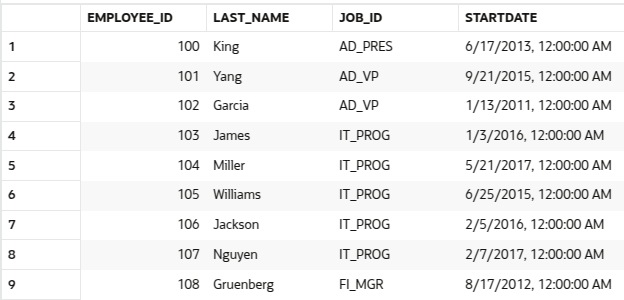
\includegraphics[scale=0.5]{images/c1q6-1.png}
\end{center}
    
\end{problem}




% ------ 7 -----------
\begin{problem}{}{problem-label}

\begin{tabular}{@{}l p{0.9\linewidth}@{}}
  \textbf{Q:} & The HR department wants a query to display all unique job IDs from the EMPLOYEES table.
\end{tabular}

\begin{center}
  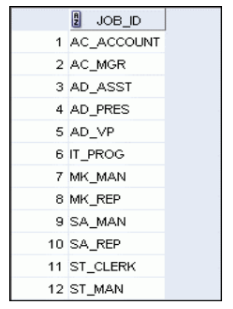
\includegraphics[scale=0.7]{images/c1q07.png}
\end{center}

\vspace{1em}

\begin{tabular}{@{}l p{0.9\linewidth}@{}}
  \textbf{A:} &
\end{tabular}

\begin{lstlisting}[language=SQL]
SELECT DISTINCT job_id
FROM hr.employees;
    \end{lstlisting}

\vspace{1em}

\begin{center}
  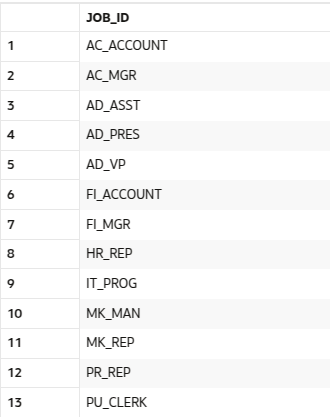
\includegraphics[scale=0.5]{images/c1a9.png}
\end{center}


\end{problem}

% ------ 8 -----------
\begin{problem}{}{problem-label}

\begin{tabular}{@{}l p{0.9\linewidth}@{}}
  \textbf{Q:} & The HR department wants more descriptive column headings for its report on employees. Copy the statement from \texttt{lab\_01\_05.sql} to a new SQL Worksheet. Name the column headings
\texttt{Emp \#}, \texttt{Employee}, \texttt{Job}, and \texttt{Hire Date}, respectively. Then run your query again.
\end{tabular}

\begin{center}
  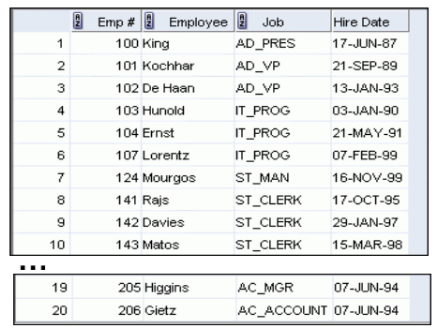
\includegraphics[scale=0.7]{images/c1q8.png}
\end{center}

\begin{tabular}{@{}l p{0.9\linewidth}@{}}
  \textbf{A:} &
\end{tabular}

\begin{lstlisting}[language=SQL]
SELECT employee_id "Emp #", 
        last_name "Employee", 
        job_id "Job", 
        hire_date "Hire Date"
FROM hr.employees;
\end{lstlisting}

\vspace{1em}

\begin{center}
  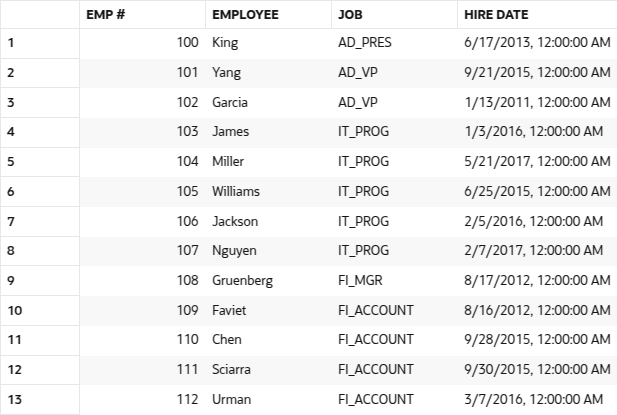
\includegraphics[scale=0.5]{images/c1a10.png}
\end{center}

\end{problem}

% ------ 9 -----------
\begin{problem}{}{problem-label}

\begin{tabular}{@{}l p{0.9\linewidth}@{}}
  \textbf{Q:} & The HR department has requested a report of all employees and their job IDs. Display the last name concatenated with the job ID (separated by a comma and space) and name the column
\texttt{EMPLOYEE} and \texttt{TITLE}.
\end{tabular}

\begin{center}
  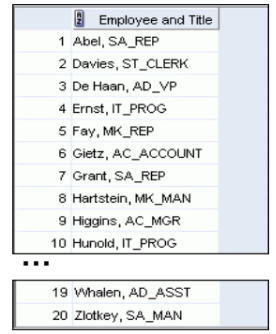
\includegraphics[scale=0.7]{images/c1q9.png}
\end{center}

\begin{tabular}{@{}l p{0.9\linewidth}@{}}
  \textbf{A:} &
\end{tabular}

\begin{lstlisting}[language=SQL]
SELECT last_name || ', ' || job_id "EMPLOYEE and EMPLOYEE"
FROM hr.employees;
\end{lstlisting}

\begin{center}
  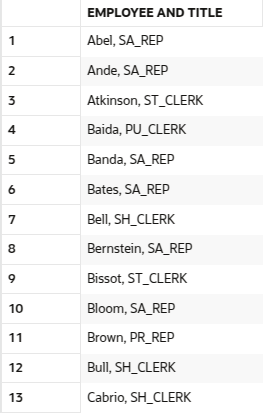
\includegraphics[scale=0.6]{images/c1a11.png}
\end{center}

\end{problem}


% ------ 10 -----------

\begin{problem}{}{problem-label}

\begin{tabular}{@{}l p{0.9\linewidth}@{}}
  \textbf{Q:} & To familiarize yourself with the data in the \texttt{EMPLOYEES} table, create a query to display all the data from that table. Separate each column output by a comma. Name the column title \texttt{THE\_OUTPUT}.
\end{tabular}

\begin{center}
  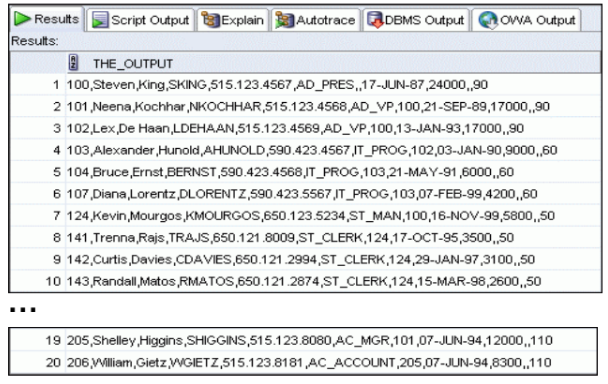
\includegraphics[scale=0.5]{images/c1q10.png}
\end{center}

\begin{tabular}{@{}l p{0.9\linewidth}@{}}
  \textbf{A:} &
\end{tabular}

\begin{lstlisting}[language=SQL]
SELECT employee_id||’,’||first_name||’,’
    ||last_name||’,’||email||’,’
    ||phone_number||’,’||hire_date||’,’
    ||job_id||’,’||salary||’,’
    ||commission_pct||’,’||manager_id||’,’
    ||department_id "THE_OUTPUT"
FROM hr.employees;
\end{lstlisting}

\begin{center}
  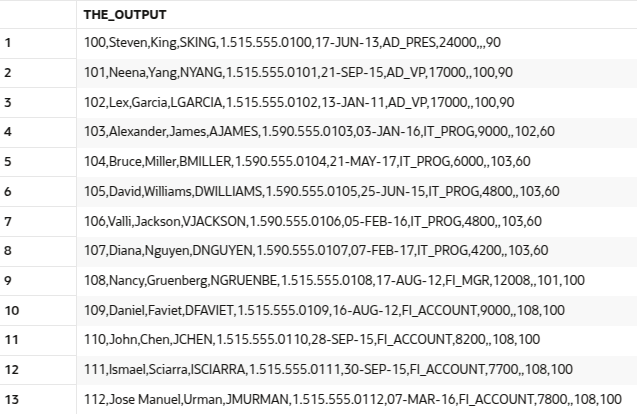
\includegraphics[scale=0.6]{images/c1a12.png}
\end{center}

\end{problem}


% ------------ Chapter 02 -----------
\newpage
\section*{Chapter 02}
\phantomsection
\addcontentsline{toc}{section}{Chapter 02: Restricting and Sorting Data}
\setcounter{problem}{0}


% ------ 1 -----------
\begin{problem}{}{problem-label}

\begin{tabular}{@{}l p{0.9\linewidth}@{}}
  \textbf{Q:} & Because of budget issues, the HR department needs a report that displays the last name and
salary of employees who earn more than \$12,000. Save your SQL statement as a file named \texttt{lab\_02\_01.sql}.. Run your query. 
\end{tabular}

\begin{center}
  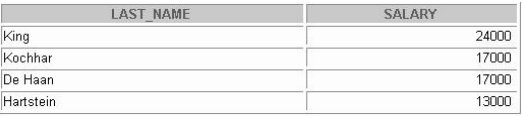
\includegraphics[scale=0.8]{images/c2q1.png}
\end{center}

\begin{tabular}{@{}l p{0.9\linewidth}@{}}
  \textbf{A:} &
\end{tabular}

\hspace{1.5em}\texttt{lab\_02\_01.sql}
\begin{lstlisting}[language=SQL]
SELECT last_name, salary
FROM hr.employees
WHERE salary > 12000;
\end{lstlisting}

\vspace{1em}

\begin{center}
  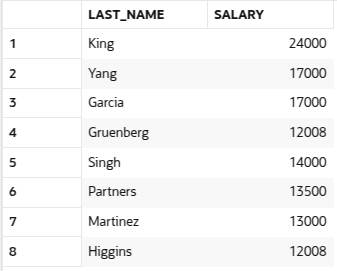
\includegraphics[scale=0.8]{images/c2a1.png}
\end{center}

\end{problem}

\newpage
% ------ 2 -----------
\begin{problem}{}{problem-label}

\begin{tabular}{@{}l p{0.9\linewidth}@{}}
  \textbf{Q:} & Create a report that displays the last name and department number for employee number 176. Run the query.
\end{tabular}

\begin{center}
  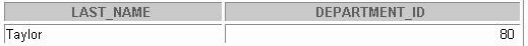
\includegraphics[scale=0.8]{images/c2q2.png}
\end{center}

\begin{tabular}{@{}l p{0.9\linewidth}@{}}
  \textbf{A:} &
\end{tabular}

\begin{lstlisting}[language=SQL]
SELECT last_name, department_id
FROM hr.employees
WHERE employee_id = 176;
\end{lstlisting}

\vspace{1em}

\begin{center}
  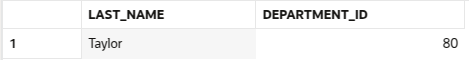
\includegraphics[scale=0.8]{images/c2a2.png}
\end{center}

\end{problem}

% ------ 3 -----------
\begin{problem}{}{problem-label}

\begin{tabular}{@{}l p{0.9\linewidth}@{}}
  \textbf{Q:} & The HR department needs to find high-salary and low-salary employees. Modify \texttt{lab\_02\_01.sql} to display the last name and salary for all employees whose salary is not in
the range of \$5,000 and \$12,000. Place your SQL statement in a text file named \texttt{lab\_02\_03.sql}.
\end{tabular}

\begin{center}
  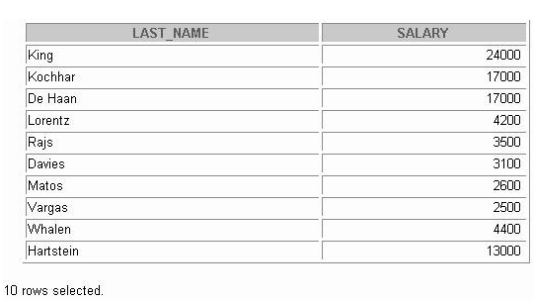
\includegraphics[scale=0.8]{images/c2q3.png}
\end{center}

\newpage

\begin{tabular}{@{}l p{0.9\linewidth}@{}}
  \textbf{A:} &
\end{tabular}

\hspace{1.5em}\texttt{lab2\_3.sql}
\begin{lstlisting}[language=SQL]
SELECT last_name, salary
FROM hr.employees
WHERE salary NOT BETWEEN 5000 AND 12000;
\end{lstlisting}

\vspace{1em}

\begin{center}
  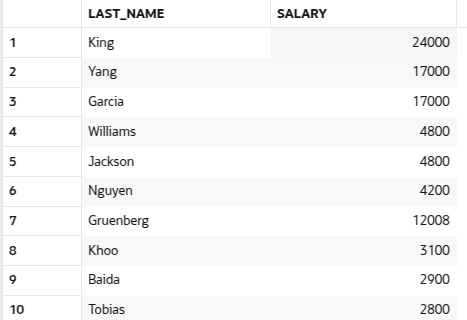
\includegraphics[scale=0.8]{images/c2a3.png}
\end{center}

\end{problem}

% ------ 4 -----------
\begin{problem}{}{problem-label}

\begin{tabular}{@{}l p{0.9\linewidth}@{}}
  \textbf{Q:} & Create a report to display the last name, job ID, and hire date for employees with the last names of Matos and Taylor. Order the query in ascending order by the hire date.
\end{tabular}

\begin{center}
  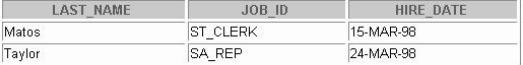
\includegraphics[scale=0.8]{images/c2q4.png}
\end{center}

\begin{tabular}{@{}l p{0.9\linewidth}@{}}
  \textbf{A:} & 
\end{tabular}

\begin{lstlisting}[language=SQL]
SELECT last_name, job_id, hire_date
FROM hr.employees
WHERE last_name IN ('Matos', 'Taylor')
ORDER BY hire_date;
\end{lstlisting}

\vspace{1em}

\begin{center}
  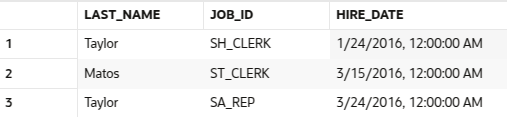
\includegraphics[scale=0.8]{images/c2a4.png}
\end{center}

\end{problem}

% ------ 5 -----------
\begin{problem}{}{problem-label}

\begin{tabular}{@{}l p{0.9\linewidth}@{}}
  \textbf{Q:} & Display the last name and department ID of all employees in departments 20 and 50 in alphabetical order by name.
\end{tabular}

\begin{center}
  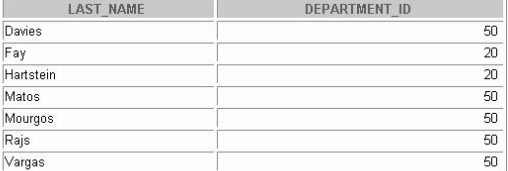
\includegraphics[scale=0.8]{images/c2q5.png}
\end{center}

\begin{tabular}{@{}l p{0.9\linewidth}@{}}
  \textbf{A:} & 
\end{tabular}

\begin{lstlisting}[language=SQL]
SELECT last_name, department_id
FROM hr.employees
WHERE department_id IN (20, 50)
ORDER BY last_name;
\end{lstlisting}

\vspace{1em}

\begin{center}
  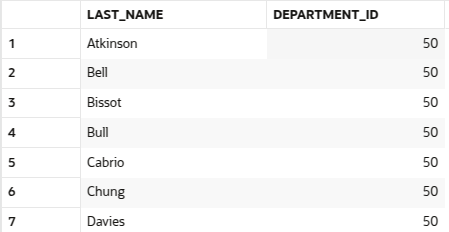
\includegraphics[scale=0.8]{images/c2a5.png}
\end{center}

\end{problem}

% ------ 6 -----------
\begin{problem}{}{problem-label}

\begin{tabular}{@{}l p{0.9\linewidth}@{}}
  \textbf{Q:} & Modify \texttt{lab\_02\_03.sql} to display the last name and salary of employees who earn between \$5,000 and \$12,000, and are in department 20 or 50. Label the columns Employee and Monthly Salary, respectively. Resave \texttt{lab\_02\_03.sql} as \texttt{lab\_02\_06.sql}. Run the statement in \texttt{lab\_02\_06.sql}.
\end{tabular}

\begin{center}
  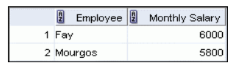
\includegraphics[scale=0.8]{images/c2q6.png}
\end{center}

\begin{tabular}{@{}l p{0.9\linewidth}@{}}
  \textbf{A:} & 
\end{tabular}

\hspace{1.5em}\texttt{lab\_02\_06.sql}
\begin{lstlisting}[language=SQL]
SELECT last_name Employee, salary "Monthly Salary"
FROM hr.employees
WHERE salary BETWEEN 5000 AND 12000
AND department_id = 20 OR department_id = 50;
\end{lstlisting}

\vspace{1em}

\begin{center}
  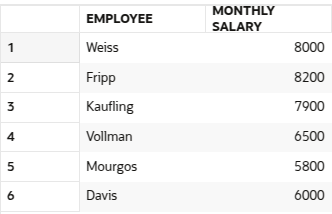
\includegraphics[scale=0.8]{images/c2a6.png}
\end{center}

\end{problem}

% ------ 7 -----------
\begin{problem}{}{problem-label}

\begin{tabular}{@{}l p{0.9\linewidth}@{}}
  \textbf{Q:} & The HR department needs a report that displays the last name and hire date for all employees
who were hired in 1994.
\end{tabular}

\begin{center}
  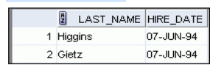
\includegraphics[scale=0.8]{images/c2q7.png}
\end{center}

\newpage

\begin{tabular}{@{}l p{0.9\linewidth}@{}}
  \textbf{A:} & \text{[Since entry os 1998 does not exist anymore we'll use 2016]}
\end{tabular}

\begin{lstlisting}[language=SQL]
SELECT last_name Employee, hire_date
FROM hr.employees
WHERE hire_date BETWEEN '1-JAN-2016' AND '31-DEC-2016';
\end{lstlisting}

\vspace{1em}

\begin{center}
  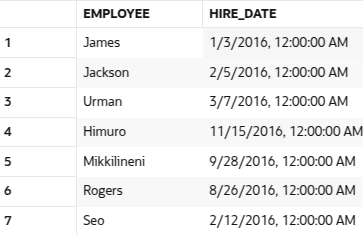
\includegraphics[scale=0.8]{images/c2a7.png}
\end{center}

\end{problem}

% ------ 8 -----------
\begin{problem}{}{problem-label}

\begin{tabular}{@{}l p{0.9\linewidth}@{}}
  \textbf{Q:} & Create a report to display the last name and job title of all employees who do not have a
manager.
\end{tabular}

\begin{center}
  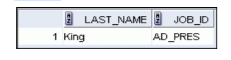
\includegraphics[scale=0.8]{images/c2q8.png}
\end{center}

\begin{tabular}{@{}l p{0.9\linewidth}@{}}
  \textbf{A:} & 
\end{tabular}

\begin{lstlisting}[language=SQL]
SELECT last_name, job_id, hire_date
FROM hr.employees
WHERE job_id = 'AD_PRES';
\end{lstlisting}

\vspace{1em}

\begin{center}
  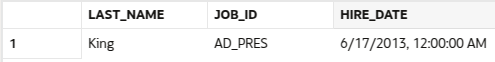
\includegraphics[scale=0.8]{images/c2a8.png}
\end{center}

\end{problem}

% ------ 9 -----------
\begin{problem}{}{problem-label}

\begin{tabular}{@{}l p{0.9\linewidth}@{}}
  \textbf{Q:} & Create a report to display the last name, salary, and commission of all employees who earn commissions. Sort data in descending order of salary and commissions. Use the column’s numeric position in the ORDER BY clause.
\end{tabular}

\begin{center}
  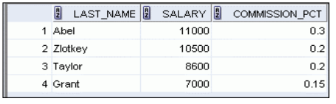
\includegraphics[scale=0.8]{images/c2q9.png}
\end{center}

\begin{tabular}{@{}l p{0.9\linewidth}@{}}
  \textbf{A:} & 
\end{tabular}

\begin{lstlisting}[language=SQL]
SELECT last_name, salary, commission_pct
FROM hr.employees
WHERE commission_pct IS NOT NULL
ORDER BY 2 DESC, 3 DESC;
\end{lstlisting}

\vspace{1em}

\begin{center}
  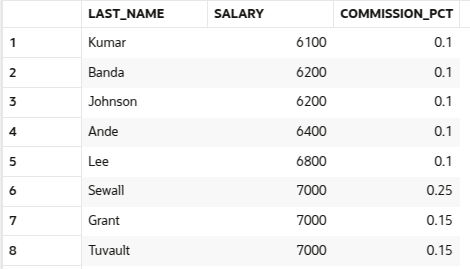
\includegraphics[scale=0.8]{images/c2a9.png}
\end{center}

\end{problem}

% ------ 10 -----------
\newpage
\begin{problem}{}{problem-label}

\begin{tabular}{@{}l p{0.9\linewidth}@{}}
  \textbf{Q:} & Members of the HR department want to have more flexibility with the queries that you are writing. They would like a report that displays the last name and salary of employees who earn more than an amount that the user specifies after a prompt. Save this query to a file named \texttt{lab\_02\_10.sql}. If you enter 12000 when prompted, the report displays the following
results:
\end{tabular}

\begin{center}
  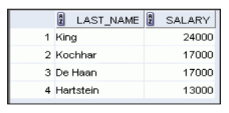
\includegraphics[scale=0.8]{images/c2q10.png}
\end{center}

\begin{tabular}{@{}l p{0.9\linewidth}@{}}
  \textbf{A:} & 
\end{tabular}

\hspace{1.5em}\texttt{lab\_02\_10.sql}
\begin{lstlisting}[language=SQL]
SELECT last_name, salary
FROM hr.employees
WHERE salary > &Salary_Amount;
\end{lstlisting}

\vspace{1em}

\begin{center}
  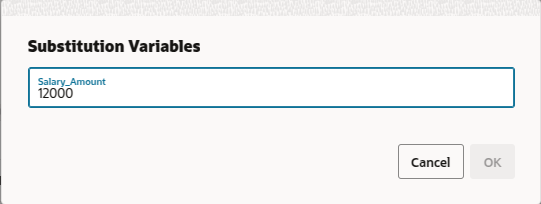
\includegraphics[scale=0.5]{images/c2a10-1.png}
\end{center}

\begin{center}
  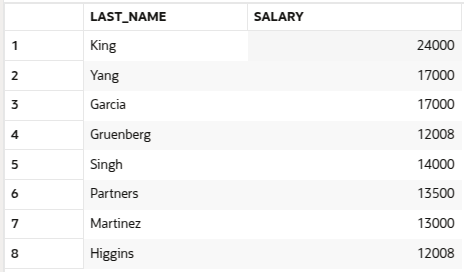
\includegraphics[scale=0.7]{images/c2a10-2.png}
\end{center}

\end{problem}

% ------ 11 -----------
\begin{problem}{}{problem-label}

\begin{tabular}{@{}l p{0.9\linewidth}@{}}
  \textbf{Q:} & The HR department wants to run reports based on a manager. Create a query that prompts the user for a manager ID and generates the employee ID, last name, salary, and department for that manager’s employees. The HR department wants the ability to sort the report on a selected column. You can test the data with the following values:
\end{tabular}

\begin{center}
  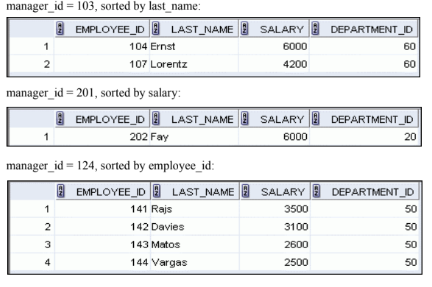
\includegraphics[scale=0.8]{images/c2q11.png}
\end{center}

\begin{tabular}{@{}l p{0.9\linewidth}@{}}
  \textbf{A:} & 
\end{tabular}

\begin{lstlisting}[language=SQL]
SELECT employee_id, last_name, salary, department_id
FROM hr.employees
WHERE manager_id = &manager_id;
\end{lstlisting}

\vspace{1em}

\begin{center}
  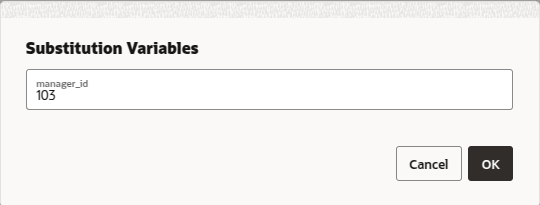
\includegraphics[scale=0.5]{images/c2a11-1.png}
\end{center}

\begin{center}
  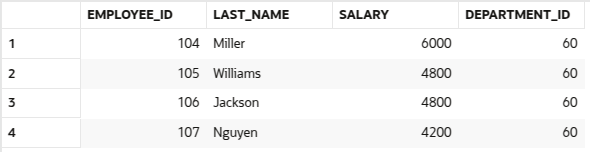
\includegraphics[scale=0.6]{images/c2a11-2.png}
\end{center}

\end{problem}

% ------ 12 -----------
\begin{problem}{}{problem-label}

\begin{tabular}{@{}l p{0.9\linewidth}@{}}
  \textbf{Q:} & Display all employee last names in which the third letter of the name is \textquote{a}.
\end{tabular}

\begin{center}
  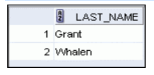
\includegraphics[scale=0.8]{images/c2q12.png}
\end{center}

\begin{tabular}{@{}l p{0.9\linewidth}@{}}
  \textbf{A:} & 
\end{tabular}

\begin{lstlisting}[language=SQL]
SELECT DISTINCT last_name
FROM hr.employees
WHERE last_name LIKE '__a%';
\end{lstlisting}

\vspace{1em}

\begin{center}
  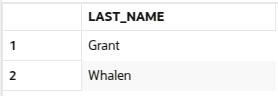
\includegraphics[scale=0.8]{images/c2a12.png}
\end{center}

\end{problem}

% ------ 13 -----------
\begin{problem}{}{problem-label}

\begin{tabular}{@{}l p{0.9\linewidth}@{}}
  \textbf{Q:} & Display the last names of all employees who have both an \textquote{a} and an \textquote{e} in their last name.
\end{tabular}

\begin{center}
  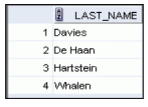
\includegraphics[scale=0.8]{images/c2q13.png}
\end{center}

\newpage

\begin{tabular}{@{}l p{0.9\linewidth}@{}}
  \textbf{A:} & 
\end{tabular}

\begin{lstlisting}[language=SQL]
SELECT DISTINCT last_name
FROM hr.employees
WHERE last_name LIKE '%a%' AND last_name LIKE '%e%';
\end{lstlisting}

\vspace{1em}

\begin{center}
  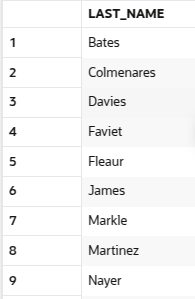
\includegraphics[scale=0.8]{images/c2a13.png}
\end{center}

\end{problem}

% ------ 14 -----------
\begin{problem}{}{problem-label}

\begin{tabular}{@{}l p{0.9\linewidth}@{}}
  \textbf{Q:} & Display the last name, job, and salary for all employees whose jobs are either those of a sales
representative or of a stock clerk, and whose salaries are not equal to \$2,500, \$3,500, or \$7,000.
\end{tabular}

\begin{center}
  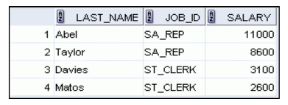
\includegraphics[scale=0.8]{images/c2q14.png}
\end{center}

\newpage

\begin{tabular}{@{}l p{0.9\linewidth}@{}}
  \textbf{A:} & 
\end{tabular}

\begin{lstlisting}[language=SQL]
SELECT last_name, job_id, salary
FROM hr.employees
WHERE (job_id ='SA_REP' OR job_id = 'ST_CLERK')
    AND salary NOT IN(2500, 3500, 7000);
\end{lstlisting}

\vspace{1em}

\begin{center}
  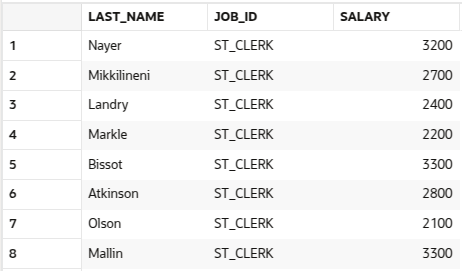
\includegraphics[scale=0.8]{images/c2a14.png}
\end{center}

\end{problem}


% ------ 15 -----------
\begin{problem}{}{problem-label}

\begin{tabular}{@{}l p{0.9\linewidth}@{}}
  \textbf{Q:} & Modify \texttt{lab\_02\_06.sql} to display the last name, salary, and commission for all employees
whose commission is 20\%. Resave \texttt{lab\_02\_06.sql} as \texttt{lab\_02\_15.sql}. Rerun the statement in \texttt{lab\_02\_15.sql}.
\end{tabular}

\begin{center}
  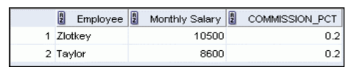
\includegraphics[scale=0.8]{images/c2q15.png}
\end{center}

\newpage

\begin{tabular}{@{}l p{0.9\linewidth}@{}}
  \textbf{A:} & 
\end{tabular}

\hspace{1.5em}\texttt{lab\_02\_15.sql}
\begin{lstlisting}[language=SQL]
SELECT last_name Employee, salary "Monthly Salary", commission_pct
FROM hr.employees
WHERE commission_pct = 0.2;
\end{lstlisting}

\vspace{1em}

\begin{center}
  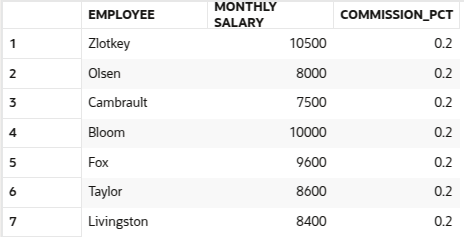
\includegraphics[scale=0.8]{images/c2a15.png}
\end{center}

\end{problem}


% ------ Chapter 03 -----------
\newpage
\section*{Chapter 03}
\phantomsection
\addcontentsline{toc}{section}{Chapter 03: Using Single-Row Functions to Customize Output}
\setcounter{problem}{0}
% ------ 1 -----------
\begin{problem}{}{problem-label}

\begin{tabular}{@{}l p{0.9\linewidth}@{}}
  \textbf{Q:} & Write a query to display the system date. Label the column as Date.
  
\textbf{Note:} If your database is remotely located in a different time zone, the output will be the date for the operating system on which the database resides.
\end{tabular}

\begin{center}
  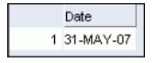
\includegraphics[scale=0.8]{images/c3q1.png}
\end{center}


\begin{tabular}{@{}l p{0.9\linewidth}@{}}
  \textbf{A:} & 
\end{tabular}


\begin{lstlisting}[language=SQL]
SELECT sysdate
FROM dual;
\end{lstlisting}


\begin{center}
  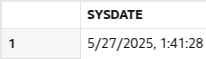
\includegraphics[scale=0.8]{images/c3a1.png}
\end{center}

\end{problem}

% ------ 2 -----------
\begin{problem}{}{problem-label}

\begin{tabular}{@{}l p{0.9\linewidth}@{}}
  \textbf{Q:} & The HR department needs a report to display the employee number, last name, salary, and
salary increased by 15.5\% (expressed as a whole number) for each employee. Label the column
New Salary. Save your SQL statement in a file named \texttt{lab\_03\_02.sql}.
\end{tabular}

\begin{tabular}{@{}l p{0.9\linewidth}@{}}
  \textbf{A:} & 
\end{tabular}

\hspace{1.5em}\texttt{lab\_03\_02.sql}
\begin{lstlisting}[language=SQL]
SELECT employee_id, last_name, salary, 
    salary+salary*0.155 "New Salary"
FROM hr.employees;
\end{lstlisting}

\vspace{1em}

\end{problem}

% ------ 3 -----------
\begin{problem}{}{problem-label}

\begin{tabular}{@{}l p{0.9\linewidth}@{}}
  \textbf{Q:} & Run your query in the \texttt{lab\_03\_02.sql} file.
\end{tabular}

\begin{center}
  \includegraphics[scale=0.8]{images/c3q3.png}
\end{center}

\begin{tabular}{@{}l p{0.9\linewidth}@{}}
  \textbf{A:} & 
\end{tabular}

\vspace{1em}

\begin{center}
  \includegraphics[scale=0.8]{images/c3a3.png}
\end{center}

\end{problem}

% ------ 4 -----------
\begin{problem}{}{problem-label}

\begin{tabular}{@{}l p{0.9\linewidth}@{}}
  \textbf{Q:} & Modify your query \texttt{lab\_03\_02.sql} to add a column that subtracts the old salary from the
new salary. Label the column \texttt{Increase}. Save the contents of the file as \texttt{lab\_03\_04.sql}.
Run the revised query.
\end{tabular}

\begin{center}
  \includegraphics[scale=0.8]{images/c3q4.png}
\end{center}

\begin{tabular}{@{}l p{0.9\linewidth}@{}}
  \textbf{A:} & 
\end{tabular}

\hspace{1.5em}\texttt{lab\_03\_04.sql}
\begin{lstlisting}[language=SQL]
SELECT employee_id, last_name, salary, 
    salary+salary*0.155 "New Salary", salary*0.155 Increase 
FROM hr.employees;
\end{lstlisting}

\vspace{1em}

\begin{center}
  \includegraphics[scale=0.5]{images/c3a4.png}
\end{center}

\end{problem}

% ------ 5 -----------
\begin{problem}{}{problem-label}

\begin{tabular}{@{}l p{0.9\linewidth}@{}}
  \textbf{Q:} & Write a query that displays the last name (with the first letter in uppercase and all the other
letters in lowercase) and the length of the last name for all employees whose name starts with the letters \textquote{J}, \textquote{A}, or \textquote{M}. Give each column an appropriate label. Sort the results by the
employees’ last names.
\end{tabular}

\begin{center}
  \includegraphics[scale=0.8]{images/c3q5-1.png}
\end{center}

\begin{tabular}{@{}l p{0.9\linewidth}@{}}
  & Rewrite the query so that the user is prompted to enter a letter that the last name starts with. For
example, if the user enters \textquote{H} (capitalized) when prompted for a letter, then the output should
show all employees whose last name starts with the letter \textquote{H}.
\end{tabular}

\begin{center}
  \includegraphics[scale=0.8]{images/c3q5-2.png}
\end{center}

\begin{tabular}{@{}l p{0.9\linewidth}@{}}
  & Modify the query such that the case of the entered letter does not affect the output. The entered
letter must be capitalized before being processed by the \texttt{SELECT} query.
\end{tabular}

\begin{center}
  \includegraphics[scale=0.8]{images/c3q5-3.png}
\end{center}

\begin{tabular}{@{}l p{0.9\linewidth}@{}}
  \textbf{A:} & 
\end{tabular}


\begin{lstlisting}[language=SQL]
SELECT INITCAP(last_name) AS "Formatted Last Name",
       LENGTH(last_name) AS "Length"
FROM hr.employees
WHERE SUBSTR(last_name, 1, 1) IN ('J', 'A', 'M')
ORDER BY INITCAP(last_name);

\end{lstlisting}

\vspace{1em}

\begin{center}
  \includegraphics[scale=0.8]{images/c3a5-1.png}
\end{center}

\begin{lstlisting}[language=SQL]
SELECT INITCAP(last_name) AS "Name",
       LENGTH(last_name) AS "Length"
FROM hr.employees
WHERE SUBSTR(last_name, 1, 1) = '&letter';
\end{lstlisting}

\vspace{1em}

\begin{center}
  \includegraphics[scale=0.5]{images/c3a5-2.png}
\end{center}
\begin{center}
  \includegraphics[scale=0.8]{images/c3a5-3.png}
\end{center}

\begin{lstlisting}[language=SQL]
SELECT INITCAP(last_name) AS "Name",
       LENGTH(last_name) AS "Length"
FROM hr.employees
WHERE SUBSTR(last_name, 1, 1) = UPPER('&letter');
\end{lstlisting}

\vspace{1em}

\begin{center}
  \includegraphics[scale=0.5]{images/c3a5-4.png}
\end{center}

\begin{center}
  \includegraphics[scale=0.8]{images/c3a5-3.png}
\end{center}

\end{problem}

% ------ 6 -----------
\begin{problem}{}{problem-label}

\begin{tabular}{@{}l p{0.9\linewidth}@{}}
  \textbf{Q:} & The HR department wants to find the duration of employment for each employee. For each employee, display the last name and calculate the number of months between today and the date on which the employee was hired. Label the column as \texttt{MONTHS\_WORKED}. Order your results by the number of months employed. Round the number of months up to the closest whole number.

\textbf{Note:} Because this query depends on the date when it was executed, the values in the \texttt{MONTHS\_WORKED} column will differ for you.
\end{tabular}

\begin{center}
  \includegraphics[scale=0.8]{images/c3q6.png}
\end{center}


\begin{tabular}{@{}l p{0.9\linewidth}@{}}
  \textbf{A:} & 
\end{tabular}


\begin{lstlisting}[language=SQL]
SELECT last_name,
       ROUND(MONTHS_BETWEEN(SYSDATE, hire_date)) AS MONTHS_WORKED
FROM hr.employees
ORDER BY MONTHS_WORKED;
\end{lstlisting}

\vspace{1em}

\begin{center}
  \includegraphics[scale=0.8]{images/c3a6.png}
\end{center}

\end{problem}

% ------ 7 -----------
\begin{problem}{}{problem-label}

\begin{tabular}{@{}l p{0.9\linewidth}@{}}
  \textbf{Q:} & Create a query to display the last name and salary for all employees. Format the salary to be 15
characters long, left-padded with the \$ symbol. Label the column as \texttt{SALARY}.
\end{tabular}

\begin{center}
  \includegraphics[scale=0.8]{images/c3q7.png}
\end{center}

\begin{tabular}{@{}l p{0.9\linewidth}@{}}
  \textbf{A:} & 
\end{tabular}


\begin{lstlisting}[language=SQL]
SELECT last_name, LPAD(salary,15,'$') AS SALARY
FROM hr.employees;

\end{lstlisting}

\vspace{1em}

\begin{center}
  \includegraphics[scale=0.8]{images/c3a7.png}
\end{center}

\end{problem}

% ------ 8 -----------
\begin{problem}{}{problem-label}

\begin{tabular}{@{}l p{0.9\linewidth}@{}}
  \textbf{Q:} & Create a query that displays the first eight characters of the employees’ last names and indicates
the amounts of their salaries with asterisks. Each asterisk signifies a thousand dollars. Sort the data in descending order of salary. Label the column as
\texttt{EMPLOYEES\_AND\_THEIR\_SALARIES}.
\end{tabular}

\begin{center}
  \includegraphics[scale=0.8]{images/c3q8.png}
\end{center}

\begin{tabular}{@{}l p{0.9\linewidth}@{}}
  \textbf{A:} & 
\end{tabular}


\begin{lstlisting}[language=SQL]
SELECT SUBSTR(last_name, 1, 8) ||'     '|| RPAD('*', ROUND(salary / 1000), '*') AS EMPLOYEES_AND_THEIR_SALARIES
FROM hr.employees
ORDER BY salary DESC;
\end{lstlisting}

\vspace{1em}

\begin{center}
  \includegraphics[scale=0.7]{images/c3a8-01.png}
  \includegraphics[scale=0.8]{images/c3a8-2.png}
\end{center}

\end{problem}

% ------ 9 -----------
\begin{problem}{}{problem-label}

\begin{tabular}{@{}l p{0.9\linewidth}@{}}
  \textbf{Q:} & Create a query to display the last name and the number of weeks employed for all employees in
department 90. Label the number of weeks column as \texttt{TENURE}. Truncate the number of weeks value to 0 decimal places. Show the records in descending order of the employee’s tenure.

\textbf{Note:} The \texttt{TENURE} value will differ as it depends on the date on which you run the query.
\end{tabular}

\begin{center}
  \includegraphics[scale=0.8]{images/c3q9.png}
\end{center}

\newpage

\begin{tabular}{@{}l p{0.9\linewidth}@{}}
  \textbf{A:} & 
\end{tabular}


\begin{lstlisting}[language=SQL]
SELECT last_name, TRUNC((sysdate-hire_date)/7, 0) AS TENURE
FROM hr.employees
WHERE department_id = 90
ORDER BY TENURE DESC;
\end{lstlisting}

\vspace{1em}

\begin{center}
  \includegraphics[scale=0.8]{images/c3a9.png}
\end{center}

\end{problem}

% ------ Chapter 04 -----------
\newpage
\section*{Chapter 04}
\phantomsection
\addcontentsline{toc}{section}{Chapter 04: Using Conversion Functions and Conditional Expressions}
\setcounter{problem}{0}

% ------ 1 -----------
\begin{problem}{}{problem-label}

\begin{tabular}{@{}l p{0.9\linewidth}@{}}
  \textbf{Q:} & Create a report that produces the following for each employee:
  
\texttt{<employee last name>} earns \texttt{<salary>} monthly but wants \texttt{<3 times salary>}. Label the column \texttt{Dream Salaries}.
\end{tabular}

\begin{center}
  \includegraphics[scale=0.8]{images/c4q1.png}
\end{center}

\begin{tabular}{@{}l p{0.9\linewidth}@{}}
  \textbf{A:} & 
\end{tabular}


\begin{lstlisting}[language=SQL]
SELECT last_name || ' earns ' || TO_CHAR(salary, 'FM$999,999') ||
    ' monthly but wants ' || TO_CHAR(salary * 3, 'FM$999,999') || '.' 
    AS "Dream Salaries"
FROM hr.employees;
\end{lstlisting}

\vspace{1em}

\begin{center}
  \includegraphics[scale=0.8]{images/c4a1.png}
\end{center}

\end{problem}

% ------ 2 -----------
\begin{problem}{}{problem-label}

\begin{tabular}{@{}l p{0.9\linewidth}@{}}
  \textbf{Q:} & Display each employee’s last name, hire date, and salary review date, which is the first Monday
after six months of service. Label the column REVIEW. Format the dates to appear in the format similar to \textquote{Monday, the Thirty-First of July, 2000}.
\end{tabular}

\begin{center}
  \includegraphics[scale=0.8]{images/c4q2.png}
\end{center}

\begin{tabular}{@{}l p{0.9\linewidth}@{}}
  \textbf{A:} & 
\end{tabular}


\begin{lstlisting}[language=SQL]
SELECT 
    last_name, 
    TO_CHAR(hire_date, 'DD-MON-YY'), 
    'MONDAY, the ' || TO_CHAR(
        NEXT_DAY(ADD_MONTHS(hire_date, 6), 'MONDAY'),
        'fmDdspth "of" Month, YYYY'
    ) AS REVIEW
FROM hr.employees;
\end{lstlisting}

\vspace{1em}

\begin{center}
  \includegraphics[scale=0.7]{images/c4a2.png}
\end{center}

\end{problem}

% ------ 3 -----------
\begin{problem}{}{problem-label}

\begin{tabular}{@{}l p{0.9\linewidth}@{}}
  \textbf{Q:} & Display the last name, hire date, and day of the week on which the employee started. Label the
column \texttt{DAY}. Order the results by the day of the week, starting with Monday.
\end{tabular}

\begin{center}
  \includegraphics[scale=0.8]{images/c4q3.png}
\end{center}

\begin{tabular}{@{}l p{0.9\linewidth}@{}}
  \textbf{A:} & 
\end{tabular}


\begin{lstlisting}[language=SQL]
SELECT 
    last_name, 
    hire_date, 
    TO_CHAR(hire_date, 'fmDay') AS DAY
FROM hr.employees
ORDER BY 
    DECODE(TO_CHAR(hire_date, 'DY', 'NLS_DATE_LANGUAGE = ENGLISH'),
        'MON', 1,
        'TUE', 2,
        'WED', 3,
        'THU', 4,
        'FRI', 5,
        'SAT', 6,
        'SUN', 7
    );
\end{lstlisting}

\vspace{1em}

\begin{center}
  \includegraphics[scale=0.8]{images/c4a3.png}
\end{center}

\end{problem}

% ------ 4 -----------
\begin{problem}{}{problem-label}

\begin{tabular}{@{}l p{0.9\linewidth}@{}}
  \textbf{Q:} & Create a query that displays the employees’ last names and commission amounts. If an employee
does not earn commission, show \textquote{No Commission}. Label the column \texttt{COMM}.
\end{tabular}

\begin{center}
  \includegraphics[scale=0.6]{images/c4q4.png}
\end{center}

\newpage
\begin{tabular}{@{}l p{0.9\linewidth}@{}}
  \textbf{A:} & 
\end{tabular}


\begin{lstlisting}[language=SQL]
SELECT last_name, 
       NVL(TO_CHAR(commission_pct), 'No Commission') AS COMM
FROM hr.employees;
\end{lstlisting}

\vspace{1em}

\begin{center}
  \includegraphics[scale=0.8]{images/c4a4-1.png}
  \includegraphics[scale=0.8]{images/c4a4-2.png}
\end{center}

\end{problem}

% ------ 5 -----------
\begin{problem}{}{problem-label}

\begin{tabular}{@{}l p{0.9\linewidth}@{}}
  \textbf{Q:} & Using the \texttt{DECODE} function, write a query that displays the grade of all employees based on the
value of the column \texttt{JOB\_ID}, using the following data:
\end{tabular}

\begin{center}
\begin{tabular}{|l|l|}
  \hline
  \textbf{\textit{Job}} & \textbf{\textit{Grade}} \\
  \hline
  \texttt{AD\_PRES} & \texttt{A} \\
  \texttt{ST\_MAN} & \texttt{B} \\
  \texttt{IT\_PROG} & \texttt{C} \\
  \texttt{SA\_REP} & \texttt{D} \\
  \texttt{ST\_CLERK} & \texttt{E} \\
  \texttt{None of the above} & \texttt{0} \\
  \hline
\end{tabular}
\end{center}

\begin{center}
  \includegraphics[scale=0.8]{images/c4q5.png}
\end{center}

\begin{tabular}{@{}l p{0.9\linewidth}@{}}
  \textbf{A:} & 
\end{tabular}


\begin{lstlisting}[language=SQL]
SELECT job_id, 
       DECODE(job_id, 'AD_PRES', 'A',
                      'ST_MAN', 'B',
                      'IT_PROG', 'C',
                      'SA_REP', 'D',
                      'ST_CLERK', 'E',
                      '0') AS GRADE
FROM hr.employees;
\end{lstlisting}

\vspace{1em}

\begin{center}
  \includegraphics[scale=0.8]{images/c4a5-1.png}
\end{center}
\begin{center}
    \includegraphics[scale=0.8]{images/c4a5-2.png}
\end{center}

\end{problem}

% ------ 6 -----------
\newpage
\begin{problem}{}{problem-label}

\begin{tabular}{@{}l p{0.9\linewidth}@{}}
  \textbf{Q:} & Rewrite the statement in the preceding exercise using the \texttt{CASE} syntax.
\end{tabular}

\begin{center}
  \includegraphics[scale=0.8]{images/c4q6.png}
\end{center}

\begin{tabular}{@{}l p{0.9\linewidth}@{}}
  \textbf{A:} & 
\end{tabular}


\begin{lstlisting}[language=SQL]
SELECT job_id, 
       CASE job_id WHEN 'AD_PRES' THEN 'A'
                   WHEN 'ST_MAN'THEN 'B'
                   WHEN 'IT_PROG'THEN 'C'
                   WHEN 'SA_REP'THEN 'D'
                   WHEN 'ST_CLERK'THEN 'E'
       ELSE        '0' END AS GRADE
FROM hr.employees;
\end{lstlisting}

\vspace{1em}

\begin{center}
  \includegraphics[scale=0.7]{images/c4a5-1.png}
\end{center}
\begin{center}
    \includegraphics[scale=0.7]{images/c4a5-2.png}
\end{center}
\end{problem}

\end{document}
